\documentclass{revtex4}
\usepackage{graphicx}
\usepackage{amsmath}
\usepackage{amssymb}
\usepackage{braket}
\usepackage{mathtools}
\usepackage{textcomp}
\usepackage{algorithm}
\usepackage{booktabs}
\usepackage{float}
\usepackage{caption}
\usepackage{color}
\linespread{2}
\begin{document}

\title{Hartree-Fock Stability Theory and its Relation to Strong Correlation}
\author{Evan Curtin}
\maketitle

\section{Goals and Relevance of Proposed Research}
    The goal of electronic structure theory is to solve the electronic Schr{\"o}dinger equation
    for a molecule or solid state system. The prevailing approach in \emph{ab initio} quantum 
    chemistry is to first compute a self-consistent single-determinant Hartree-Fock (HF) solution 
    which will serve as a reference for many-body perturbative (MP) or coupled-cluster (CC) 
    approaches.  
    Implicit in these methods is the assumption that the reference wave function will be 
    sufficiently close to the exact solution of the Schr{\"o}dinger equation to converge to the 
    correct 
    answer in a computationally feasible manner. Both the MP and CC approaches have the attractive 
    quality that they are systematically improvable, i.e. increasing the accuracy of the resulting 
    solution can be done by using a higher order of the theory. These so-called post-Hartree-Fock 
    methods are able to recover more of the total electronic energy by accounting for the 
    \emph{correlation energy} in the system. Traditionally, the correlation energy is defined by 
    the difference between the exact energy and the Hartree-Fock energy \cite{Shavitt2009}
    \begin{equation}\label{correlation_energy}
      E_{corr} = E_{exact} -  E_{HF}
    \end{equation}
    In many cases the correlation energy is relatively small and the Hartree-Fock reference 
    captures a significant portion of the exact total energy. In such cases, the prevailing 
    approach is usually successful and has only implementation issues for larger systems. On the 
    other hand there are systems which are not well treated by this approach, which are often 
    called ``strongly correlated''. Examples of such systems are those with degenerate or 
    near-degenerate HOMO-LUMO gaps, metallic solids or molecules close to breaking bonds. 
    Oftentimes for such systems the traditional Hartree-Fock solutions are not even qualitatively 
    correct, implying inadequacies in either the single-reference or mean-field approach. 
      
      It is often neglected, however, that the usual way for computing a Hartree-Fock solution in 
      practice
    is to use a restricted form of the single determinantal wavefunction. In the Restricted 
    Hartree-Fock (RHF), the wave function is restricted to be an eigenfunction of the $\hat{S^2}$ 
    and $\hat{S_z}$ 
    operators, while in the Unrestricted variant (UHF), the wave function need only be an 
    eigenfunction 
    of the $\hat{S_z}$. There is yet another lesser-known variation of the theory, known as General 
    Hartree-Fock (GHF), which assumes no spin-symmetries in the wave function. This allows for 
    greater
    variational flexibility at the cost of ``broken symmetry''. Together these three levels of 
    Hartree-Fock theory form a heirarchy of increasing parameter space within which to minimize the 
    total energy. Thus the term ``Hartree-Fock Energy'' is inherently ambigious; this fact calling 
    into question commonly held ideas about correlation and Hartree-Fock theory. Take for example 
    the dissociation curve of H$_2$ in the RHF and UHF approximations, compared with the exact 
    solution obtained by full configuration-interaction in the complete basis set limit. 
    
    \begin{figure}[H]
      \centering
      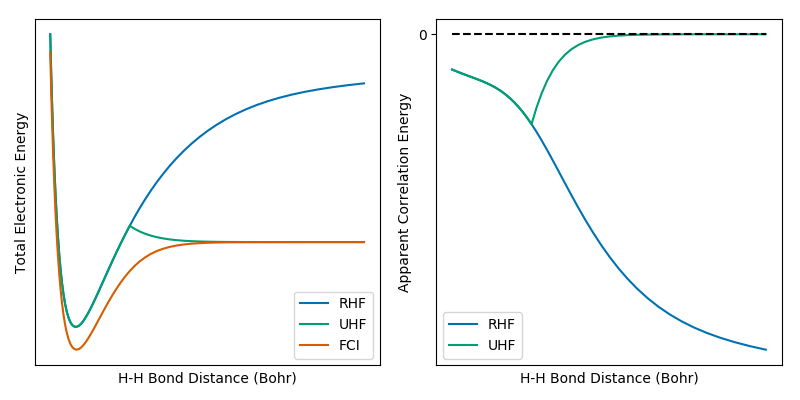
\includegraphics[width=0.75\textwidth]{../figures/H2_curves.png}
      \caption{Dissociation curve of H$_2$ in the RHF and UHF approximations, compared to the 
               exact limit (FCI). The difference in correlation energies as determined by 
               each reference illustrates the ambiguity of that quantity. In the             
               dissociation limit, the UHF correlation energy vanishes while the RHF
               correlation energy increases in magnitude.}
      \label{h2diss}
    \end{figure}
    
    The correlation energy for the RHF reference case is dramatically larger than that for the UHF 
    reference. In other words, \emph{the correlation energy is, by definition, inherently coupled 
    to the 
    Hartree-Fock reference}. The given example is well understood, but it brings to mind a more 
    general idea that there may be more cases where apparently large correlation energies are due 
    to simply 
    using and inadequate level of Hartree-Fock theory. Scuseria and coworkers have leveraged this 
    idea to create new coupled cluster theories while preserving the symmetry of the reference 
    \cite{Gomez2016}. 
    
    Another approach to this problem is to allow breaking of symmetry, and to take the variational 
    principle at face value; lower 
    energy is 
    always better. For predicting certain observables this is not the case, but for energies alone 
    we are free 
    to maintain this mindset. If the HF solution is allowed to relax fully in its most general 
    form, the resulting correlation energy may be reduced dramatically. Therefore the overarching 
    theme of the proposed work is that 
    \emph{many 
    examples of strong correlation may be misleading, and in order to find out we have to find 
    lower 
    energy Hartree-Fock solutions, even at the cost of broken symmetry}.    
    
    For some time an approach to find lower energy HF solutions has been known to follow the 
    instability eigenvectors down in energy 
    to find lower energy solutions \cite{Seeger1977}. This approach will, by construction, always 
    lead to a lower energy HF solution than the starting point. However, it is important to 
    remember that the instability condition is a local phenomena, and the lower energy solution is 
    not itself guaranteed to be the \emph{lowest} energy solution. The standard approach still 
    suffers 
    from the global optimization problem: whether a solution is a local or global minimum can only 
    be known by comparing it to the other minima of the surface. In fact, the problem of finding 
    the lowest energy HF solution has a direct correspondence to the problem of finding minimum 
    energy points on a potential energy surface of atomic coordinates. It is therefore proposed to 
    adopt approaches from that field to apply to the current problem. An attractive approach is the 
    Global Reaction Route Mapping (GRRM) method with its Anharmonic Downward Distortion (ADD) 
    algorithm \cite{Ohno2006, Ohno2016}. 
    
    \begin{figure}
      \centering
      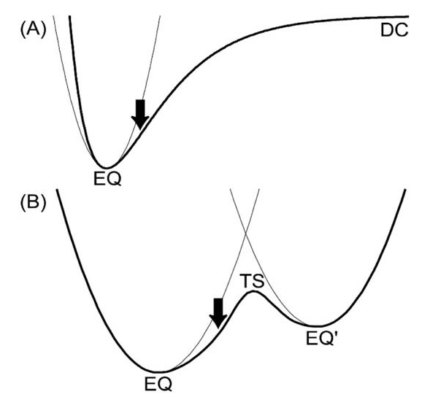
\includegraphics[width=0.5\textwidth]{../figures/ADD.png}
      \caption{Example PES illustrating the ADD effect. A) The anharmonicity increases in the 
      direction towards flattening of the PES due to dissociation (DC). B) The anharmonic 
      distortion of the 
      harmonic potential points in the direction from one equilibrium point to another. Taken from 
      Ohno\cite{Ohno2016}.}
      \label{add}
    \end{figure}
    
    In essence, the algorithm leverages the idea that the 
    presence of a local minimum influences the surrounding energy landscape (in a smooth surface). 
    The minimum will lower the energy pathways leading towards it, and softens the ascent of energy 
    around a transition state. This softening of the PES can be seen by increased anharmonicity in 
    the PES's Taylor expansion (see Fig.~\ref{add}). Thus a waypoint from one minimum to another 
    can 
    be determined by 
    finding the direction with the highest anharmonicity, and these can be followed to find new 
    solutions. By adopting this approach to use 
    molecular orbital expansion 
    coefficients in place of normal mode coordinates, many minima of the Hartree-Fock electronic 
    energy surface can be found. The proposed algorithm would have the following steps. First, a HF 
    calculation will be performed and solved self-consistently to find a stationary point. This 
    solution will then be subject to the stability analysis. If the solution is unstable, the 
    instability eigenvector will be followed downhill and a new solution will be found. This will 
    be repeated until a local minimum solution is found. Once this has been completed, the ADD 
    algorithm can be applied to the minimum solution to search for the direction of other minima 
    using the HF stability eigenvectors (the electronic analogue to vibrational modes). We then 
    perturb our solution in that direction and repeat the process to search for all relevant 
    minima. 
    
    \begin{figure}
      \centering
      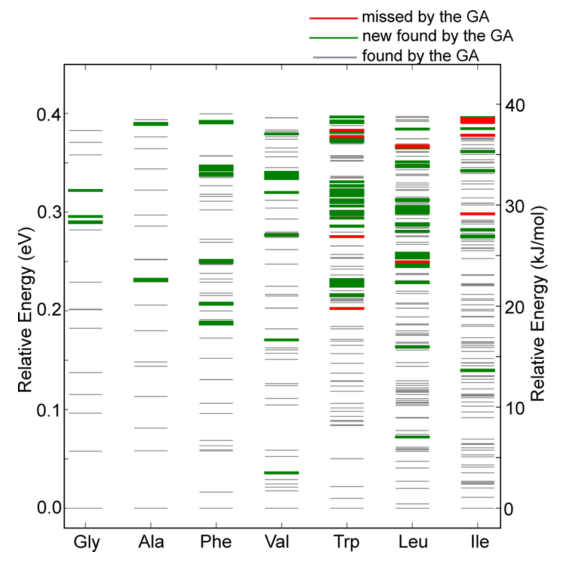
\includegraphics[width=0.4\textwidth]{../figures/GA_supady.png}
      \caption{Conformations of dipeptides found in a search using a Genetic Algorithm. The GA 
      results were compared to a reference data set. Taken from Supady~\cite{Supady2015}. Note that 
      the only missed conformations are relatively higher-energy.}
      \label{GA}
    \end{figure}  
    
    In the event that the ADD algorithm doesn't perform well, there is another option that requires 
    no assumptions about the underlying potential energy surface. The Genetic Algorithm is a 
    machine learning technique that has been applied to search for minimum energy conformations in 
    peptide dimers~\cite{Supady2015}. Genetic algorithms have seen use in various global 
    optimization problems, and have been designed via mutation to avoid being stuck in local 
    minima. This makes them well suited for finding a host of high-fitness solutions (see 
    Fig.~\ref{GA}). This approach could be implemented by using the GHF initial guess density 
    matrix as a gene 
    for the algorithm, and a fitness function which prioritizes low-energy HF solutions in a manner 
    similar to the method of Supady~\cite{Supady2015}. 
    
    If effective, either the ADD or the Genetic   algorithm could then be used to investigate 
    strong 
    correlation of various systems. If it 
    turns out that fully minimizing the HF energy can reproduce a majority of the ``correlation 
    energy'' in these systems, then using this HF searching method becomes a justified method of 
    solving strongly correlated systems. This would mean that the strong correlation was in fact illusory, and is convertible to a weak correlation problem by means of a more rigorous Hartree-Fock theory. 
    
    Another topic of interest is the metal-insulator transition in infinite systems. For a 
    particular type of insulator, the Mott Insulator, the transition from the metallic phase to the 
    insulating phase is due to emergence of a Spin Density Wave (SDW). The SDW is oscillating 
    density of up and down spins throughout space in a checkerboard pattern. The presence of a 
    gapped Mott insulator phase in high-$T_c$ cuprates (which is not predicted by band 
    theory) hints at 
    a connection between Mott insulators and some superconducting materials, but this is not fully 
    understood. Again the finite 
    systems may give clues to 
    explain under what circumstances (Temperature, Pressure, dopant concentration) this transition 
    occurs. Since HOMO-LUMO degeneracy in RHF solutions of finite systems is accompanied by a 
    triplet instability, the emergence of triplet instability can serve as a proxy for an RHF-UHF 
    transition. The corresponding corollary for the solid state case is that triplet instability 
    can signal a paramagnetic-SDW transition. Therefore we can calculate the instability as a 
    function of temperature, pressure and dopant concentration to map out a metallic / insulating 
    phase diagram for infinite systems. A temperature-dependent periodic Hartree-Fock has already 
    been developed and applied to a 2D hydrogen sheet (by other members of the Hirata Lab), a crude 
    but reasonable starting point for testing this approach. By varying the dimensionality, 
    temperature and pressure of the hydrogen sheet, we can monitor the UHF instability and 
    determine under what circumstances the SDW phase becomes present at higher temperatures. In 
    doing so, we hope to be able to understand further how to create new materials with controlled 
    Mott-Insulating transitions, which may be related to increasing the $T_c$ of superconducting 
    materials (See Fig.~\ref{scphase}). 
    
    \begin{figure}
       	\centering
       	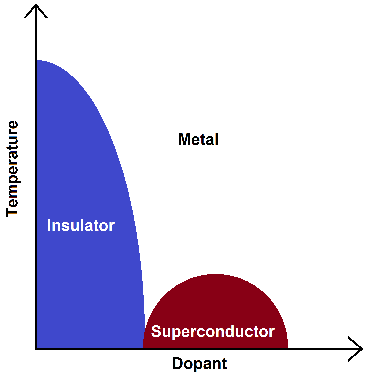
\includegraphics[width=0.3\textwidth]{../figures/NSFdiagram.png}
       	\caption{Cartoon illustration of a phase diagram of superconducting transitions. The insulator (SDW) phase is thought to increase with the superconducting phase.}
       	\label{scphase}
    \end{figure}
    
    
\newpage

\section{Accomplishments}

   
   \subsection{Hartree-Fock Stability}
    Hartree-Fock (HF) Theory has been the foundation for \emph{ab initio} electronic structure 
    theory 
    throughout its history. An often overlooked aspect of the theory is that there are many 
    solutions to the HF equations for a given system, but being a 
    solution to the Hartree-Fock equation ensures only that the solution is stationary with respect 
    to the 
    determined orbitals. If the solution is indeed a minimum, it is called ``stable'', while if 
    there 
    is any displacement in the electronic structure which lowers the energy, the solution is 
    ``unstable''. A method for determining the stability of a Hartree-Fock solution was 
    proposed by Thouless in 1960\cite{Thouless1960}. The condition was rederived into the 
    expression familiar to quantum chemists by Čížek and Paldus in 1967\cite{Cizek1967}. 
    Furthermore, the stability equations factorize depending on the symmetry of the Hartree-Fock 
    eigenfunctions. To this end, Seeger and Pople outlined a hierarchical approach to 
    systematically evaluate the stability of HF states in the restricted, unrestricted and 
    generalized Hartree-Fock procedures\cite{Seeger1977}. Recently, the method has been used to aid 
    the search for the lowest-energy Unrestricted Hartree-Fock (UHF) solutions in molecules, as 
    well as the General Hartree-Fock (GHF) solutions in geometrically frustrated hydrogen rings 
    which cannot conform even to the UHF scheme\cite{Pulay2016, Goings2015}. The lower energy HF 
    solutions in these studies were located by first finding the instabilities in the higher 
    spin-symmetry solutions, then using this information to obtain ``symmetry breaking'' 
    displacements that lower the energy.
    
    To determine if there is indeed a symmetry-broken HF solution of lower energy, the usual method 
    is to determine the stability of a found Hartree-Fock solution. Instabilities are indicated by a
    negative
    eigenvalue the Electronic Hessian, 
    \begin{equation}
     \bf{H}=
     \begin{bmatrix}
     \bf{A} &\bf{B} \\
     \bf{B}^* & \bf{A}^* \\
     \end{bmatrix},
    \end{equation} 
    where the matrices $\mathbf{A}$ and $\mathbf{B}$ have dimension $N_{occupied} \times 
    N_{virtual}$ with elements given by
    \begin{align}
     A_{i \rightarrow a, j \rightarrow b} &= (\epsilon_a-\epsilon_i)\delta_{ij}\delta_{ab} 
     + \left< aj||ib \right>, \\
     B_{i \rightarrow a, j \rightarrow b} &= \left< ab||ij \right>. 
    \end{align}    
    For a paramagnetic HF solution (RHF), the Orbital Hessian
    factorizes into the matrices known to 
    chemists as the singlet and triplet instability matrices ($\bf{{}^1H}$ and $\bf{{}^3H}$, 
    respectively)\cite{Dunning1967,Seeger1977}.
    
     \begin{subequations}
     	\begin{align}
     	{}^{1}{A'}_{i\rightarrow a, j\rightarrow b} &= (\epsilon_a-\epsilon_i)\delta_{ij}\delta_{ab} 
     	+ 2\braket{aj|ib}-\braket{aj|bi}\\
     	{}^{3}{A'}_{i\rightarrow a, j\rightarrow b} &= (\epsilon_a-\epsilon_i)\delta_{ij}\delta_{ab} 
     	- \braket{aj|bi}\\
     	{}^{1}{B'}_{i\rightarrow a, j\rightarrow b} &= 2\braket{ab|ij}-\braket{ab|ji}\\
     	{}^{3}{B'}_{i\rightarrow a, j\rightarrow b} &= -\braket{ab|ji}
     	\end{align}
     \end{subequations}
      The lowest eigenvalue of both of 
     these matrices will reveal the stability of the RHF solution. If  ${}^1\bf{H}$ has negative 
     eigenvalues, the
     solution is unstable with respect to changes that preserve singlet character (singlet 
     instability), while if ${}^3\bf{H}$ has negative eigenvalues, the solution is unstable towards 
     displacements that would change the wavefunction towards a triplet state (triplet 
     instability). The solution is stable if neither ${}^1\bf{H}$ nor ${}^3\bf{H}$ has a negative 
     eigenvalue. An 
     eigenvalue of 0 does not indicate instability, and this case is discussed 
     in detail by Cui et al \cite{Cui2013}.
    
    \subsection{Hartee-Fock Stability of the Homogeneous Electron Gas}
    
    Previously it has been shown for finite systems with form-degenerate HOMO-LUMO, there always 
    exists a symmetry-breaking instability\cite{Yamada2015}. Whether this theorem holds in the 
    infinite case remains to be seen. To investigate HF instabilities in zero band gap solids, a 
    natural starting point is the Homogeneous Electron Gas (HEG, often called Jellium or Uniform 
    Electron Gas) model. The model consists of electrons in a box with periodic boundary conditions 
    and the constraint that the entire system is charge-neutral via a uniform background positive 
    charge. The resulting Coulomb interactions cancel exactly, and the only remaining terms are due 
    to kinetic and exchange energies. Historically it was thought that the 
    plane-wave paramagnetic solution to the HF equations for this model was the ``correct'' 
    solution. However, in a landmark paper, Overhauser showed that certain symmetry broken 
    solutions \emph{always} have lower-energy than the paramagnetic solutions at all electron 
    densities\cite{Overhauser1962}. This hints at, but does not show, that the analogous triplet 
    instability theorem persists in the infinite case.  
    
      Overhausers' paper sparked new interest in the HEG, and since then Energies of various 
      phases thereof 
      have been computed to great 
    accuracy\cite{Ceperley1980}. More 
    recently, phase diagrams have been determined for the 
    HEG in 2 and 3 dimensions\cite{Delyon2008, Bernu2011, Baguet2013}. In all cases the 
    phase diagrams are made by computing the energies of the polarized and unpolarized states, and 
    comparing them. This approach necessitates that the form of the solutions is known ahead of 
    time. 
    
    The present work focuses on directly calculating the Hartree-Fock stability of 
    the 
    paramagnetic homogeneous electron gas as a function of electron density. The motivation is 
    two-fold. First, the numerical studies of this model can give computational evidence for or 
    against the ubiquity of symmetry-breaking HF instabilities in metallic solids. Secondly, the 
    instabilities can help in determining lower energy HF solutions of the HEG. This is because the 
    study will reveal where the symmetry broken Hartree-Fock reference is needed. To date, an 
    optimal form (i.e. minimal energy in the HF manifold) of the Hartree-Fock solution to the HEG 
    remains unknown, even though exact energy 
    (including correlation) is essentially known. Therefore determining a lower energy HF solution 
    can yield insight into the effects of correlation of this fundamental physical model. 
    	
  \subsection{Method}

	Starting with the Jellium Hamiltonian in atomic units, 
	\begin{equation}\label{hamiltonian}
		\hat{H} = \sum_i \frac{\hat{p}_i^2}{2}  + \frac{1}{2} \sum_{i < j} \frac{1}{|\vec{r}_i - 
		\vec{r}_j|},
	\end{equation}
	one solution to the Hartree-Fock equations in $D$ dimensions are plane waves of the form	
	\begin{equation}\label{planewave}
		\phi_{\vec{k}} =
		   \frac{1} { \sqrt{L ^ D} } e ^ {i \vec{k} \dot \vec{x}},
	\end{equation}
	where $L$ is the length of one side of the direct lattice with cubic symmetry. Using this as the 
	basis for the rest of the analysis, the two electron repulsion integrals are analytic and 
	well-behaved in two and three dimensions\cite{Delyon2008, Guiliani2005}
  \begin{align}
   	\braket{\vec{k}, \vec{k}' | \vec{k}'', \vec{k}'''} 
  	  \stackrel{ \text{2D, 3D} }{=}&
   	\begin{cases} 
   	\frac{\pi} {L ^ D} \frac{ 2^{D-1} } { | \vec{k} - \vec{k}'' | ^ {D-1} } 
   	& \vec{k}''' = \vec{k} + \vec{k}' - \vec{k}'' + n\vec{G} \textbf{ and } | \vec{k} - 
   	\vec{k}''| \neq 0 \\
   	0 
   	& \text{else},
   	\end{cases}
  \end{align}
  where $n\vec{G}$ is any integer times a reciprocal 
  lattice vector of the 
  system. The orbital energies are
  \begin{equation}\label{eq:hf_orb_energy}
  \epsilon_{\vec{k},\sigma}=
  \frac{\hbar^2\vec{k}^2}{2m} - \sum\limits_{\vec{k}}^{|\vec{k}|< 
  k_f}n_{\vec{k}\sigma}\braket{\vec{k}, \vec{k}' |\vec{k}', \vec{k}},
  \end{equation}
  where $n_{\vec{k}\sigma}$ is the occupation number of the state with momentum $\vec{k}$ and 
  spin $\sigma$ \cite{Guiliani2005}. In one dimension, the two electron integral diverges, and it 
  is common to use a delta function interaction, 
  \begin{equation}
    V(r_{12}) = V_0\delta(r_{12}),
  \end{equation}
  and the two electron integral in this case is simply
  \begin{align}
   	\braket{\vec{k}, \vec{k}' | \vec{k}'', \vec{k}'''} 
  	  \stackrel{ \text{1D} }{=}&
   	\begin{cases} 
   	V_0 
   	& \vec{k}''' = \vec{k} + \vec{k}' - \vec{k}'' + n\vec{G}\\
   	0 
   	& \text{else}.
   	\end{cases}
  \end{align}  
    
 \subsection{Results}   
      Using the equations for energies and two electron integrals, the stability analysis was 
      performed on the paramagnetic HEG model as a function of electron density (or equivalently, 
      the Wigner-Seitz radius, 
      $r_s$). The naive approach of explicitly constructing and diagonalizing the orbital hessian 
      is intractable both in terms of memory and calculation time requirements. Since the 
      instability condition is that the any eigenvalue is negative, it suffices to calculate the 
      sign of only the lowest eigenvalue. This is a task well suited for an iterative subspace 
      solver. To this end, a parallel version of the Jacobi-Davidson algorithm 
      was implemented by representing the matrix as a matrix-vector product (made possible by the 
      SLEPc library\cite{Hernandez2005}). This allowed for two necessary optimizations. First, the 
      algorithmic change from full diagonalization to a subspace algorithm reduces the memory 
      requirements from $O(N^2)$ to $O(N)$ and the computational scaling from $O(N^3)$ to $O(N^2)$ 
      (See Fig.~\ref{fig:scaling}). 
      Secondly, the parallelization of the algorithm allows the program to be run on the Blue 
      Waters supercomputer with about 80\% strong parallel scaling efficiency 
      (Fig.~\ref{fig:parallel}). 

     
      \begin{figure}[t]
        \begin{minipage}[c]{0.45\linewidth}
          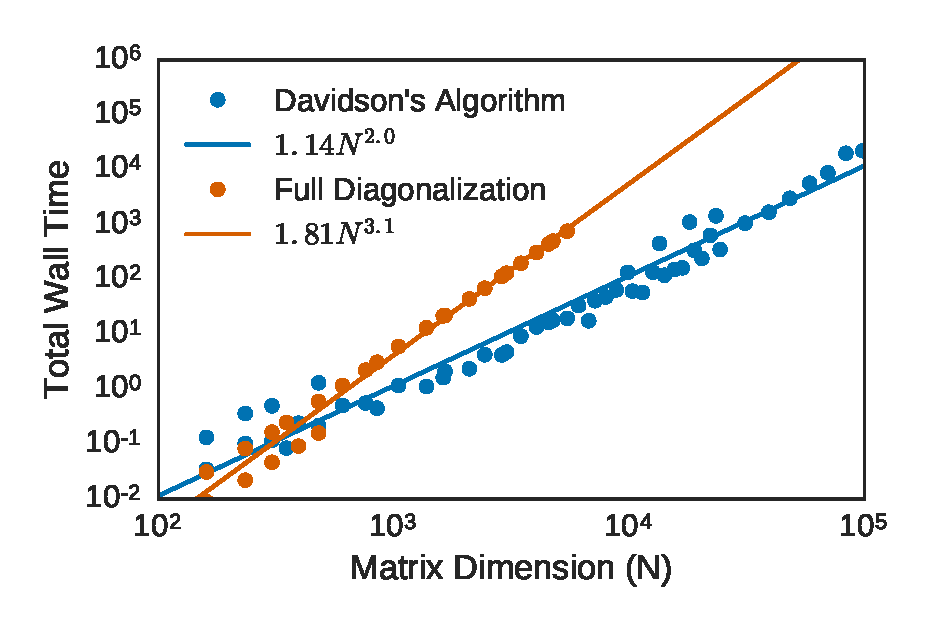
\includegraphics[height=0.7\linewidth]{../figures/dav_vs_exact_scaling.eps}
          \caption{The asymptotic scaling of both algorithms behaves as expected.}
          \label{fig:scaling}
        \end{minipage}
        ~
        \begin{minipage}[c]{0.45\linewidth}
          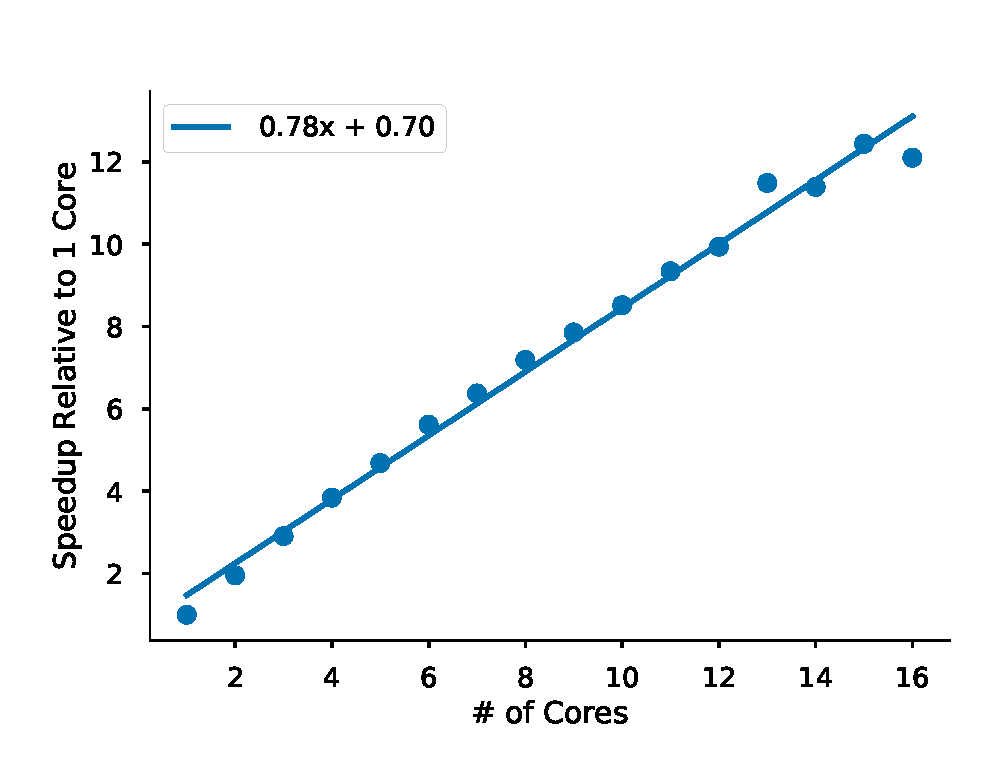
\includegraphics[height=0.7\linewidth]{../figures/parallel-scaling.eps}
          \caption{The speedup of the entire calculation as the number of computer cores is 
                          sufficiently linear.}
          \label{fig:parallel}
        \end{minipage}%
      \end{figure}
     
     
     These optimizations allow the calculation to be performed with enough grid points to converge 
     the resulting ``transition $r_s$'', the Wigner-Seitz radius at which the HF solution 
     transitions 
     from stable to unstable.          
      \begin{figure}[H]
      \centering
        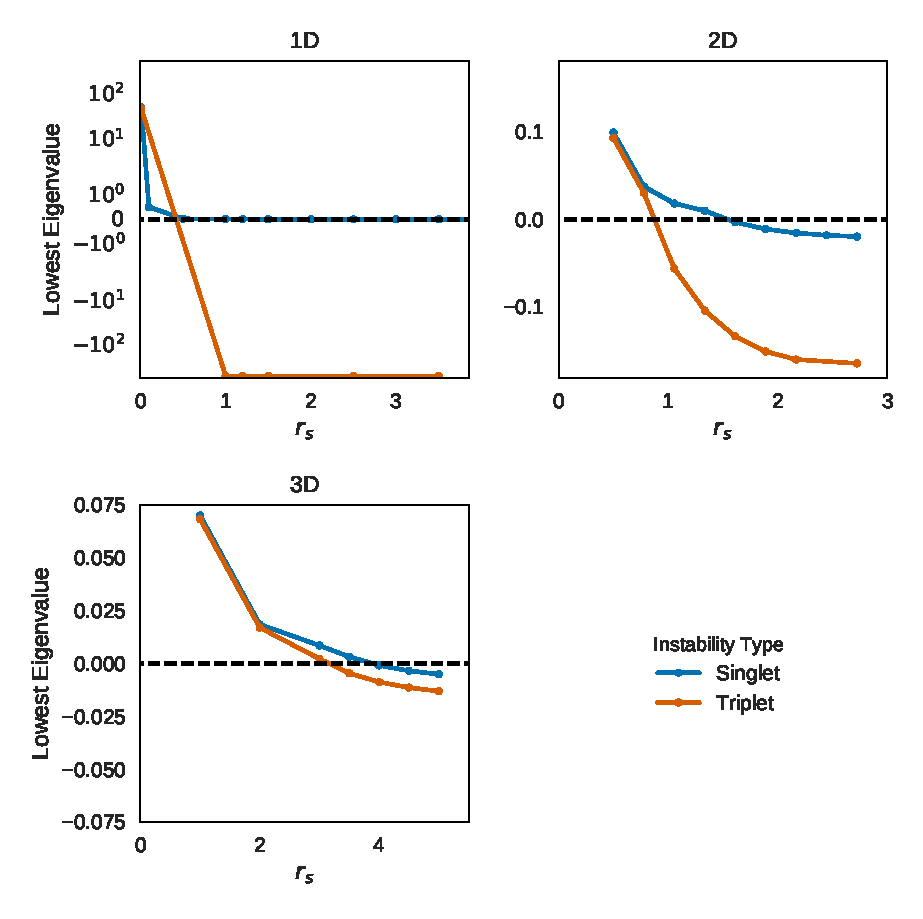
\includegraphics[width=\textwidth]{../figures/stability.eps}
        \caption{The Lowest eigenvalues of the triplet and singlet instability matrices in 1, 2 and
        3 dimensions.}
        \label{fig:stability}
      \end{figure}   
        
    The transition $r_s$ occurs at $r_s = 1$ in 2D and $r_s = 3$ in 3D (See 
    Fig.~\ref{fig:stability} and Fig.~\ref{fig:onset}). These 
    results are consistent with those seen by other methods\cite{Baguet2014, Bernu2011}. On 
    the other hand, the transition 
    $r_s$ for one dimension tends towards zero and stays quite close as the number of gridpoints 
    increases. Indeed, numerical issues appear at very high density (low $r_s$) due to divergence 
    of the two electron integrals in the asymptotic limit. With this in mind, it is clear at least 
    that the instability in the 1D case persists even at very high densities (potentially all 
    finite densities), which is to be expected from Overhauser's proof of instability at all 
    values of $r_s$ in 1D for the delta function potential \cite{Overhauser1962}.


    \begin{figure}[H]
    \centering
      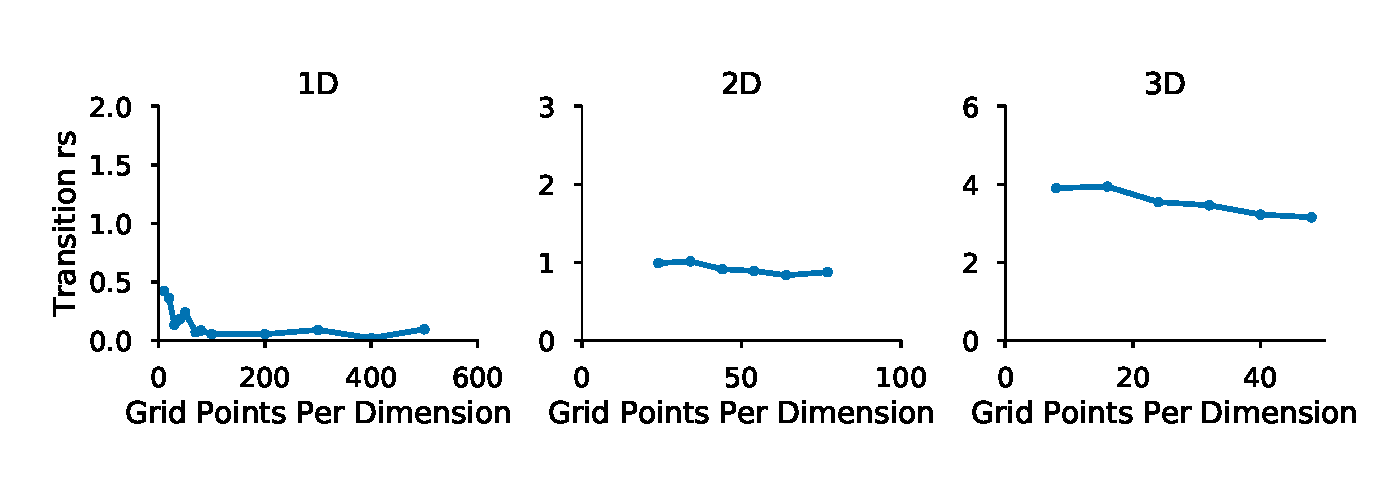
\includegraphics[width=\textwidth]{../figures/triplet_onset.eps}
      \caption{The value of $r_s$ at which the triplet instability occurs with increasing number of 
      k-points in 1, 2 and 3 dimensions.}
      \label{fig:onset}
    \end{figure}
    
      
\newpage
\section{References}
\bibliography{../prelim_references}

\end{document}